\section{Radioactivity: Doses}

%\frame{\tableofcontents[currentsection]}

\begin{frame}{Exposure (X)}

\alert{Definition}:  is a measure of the ionization of air due to ionizing radiation from photons, that is, gamma rays and X-rays.  It is defined to be the electric charge freed by the radiation divided by the mass of the air.

\alert{Units}: coulomb per kilogram, however the roentgen is commonly used internationally in the nuclear industry (1R $\sim$ 3876 C kg$^{-1}$)

\end{frame}

\begin{frame}{Exposure rate constant}

\alert{The gamma ray field can be characterized by the exposure rate}



\[X=\frac{\Gamma\cdot A}{r^2}\]




\begin{itemize}
\item $X$: exposure rate (R h$^{-1}$)
\item $\Gamma$: exposure rate constant
\item $A$: activity 
\item $r$: distance 
\end{itemize}


\end{frame}



\begin{frame}{Exposure rate constants for various radionuclides}

\begin{table}[H]
%\caption{}
%\label{tab::}
\vskip -0.5cm
\begin{center}
  \begin{tabular}{p{3cm}p{3.8cm}}
  \toprule
  Radionuclide & Exposure rate constant (	R cm$^2$ h$^{-1}$ mCi$^{-1}$)  \\ \otoprule
$^{60}$ Co & 12.838 \\
$^{99}$Mo & 1.03\\
$^{99m}$Tc & 0.720\\
$^{137}$Cs & 3.400\\
$^{226}$Ra & 8.25
  \\ \bottomrule
\end{tabular}
\end{center}
\end{table}

\end{frame}

\begin{frame}{Absorbed dose (D)}

\alert{Definition}: the mean energy imparted to matter per unit mass by ionizing radiation

\alert{Units}:  joules per kilogram  (gray, Gy)

\vskip1cm

\setbeamercolor{boxsthlmBlue}{bg=\cnLightGreen, fg=\cnPurple}\begin{beamercolorbox}[wd=\linewidth,ht=12ex,dp=3ex]{boxsthlmBlue}\centering 1 Gy = 1 J kg$^{-1}$

1 Gy = 100 rad

1 rad = 0.01 Gy = 10 mGy\end{beamercolorbox}






\end{frame}


\begin{frame}{Exposure and absorbed dose}


\[D = f \cdot X\]



f: conversion coefficient depending on medium


\alert{The absorbed energy in a quantity of air exposed to 1 C kg$^{-1}$ of X Rays is 0.869 Gy
$f$(air) = 0.869}

\begin{table}[H]
\caption*{Conversion coefficients (\emph{Credit: IAEA})}
%\label{tab::}
\vskip 0.2cm
\begin{center}
  \begin{tabular}{llll}
  \toprule
  Photon energy (keV) & $f$ water & $f$ bone  & $f$ muscle \\ \otoprule
10 & 0.91 & 3.5 & 0.93 \\
100 & 0.95 & 1.5 & 0.95  \\ \bottomrule
\end{tabular}
\end{center}
\end{table}

\end{frame}

\begin{frame}{Equivalent dose (H)}

\alert{Definition}: is the absorbed dose multiplied by a dimensionless radiation weighting factor, wR which expresses the biological effectiveness of a given type of radiation

\alert{Units}: the SI unit of equivalent dose is called the sievert (Sv). The old unit was the ``rem''

\vskip1cm

\setbeamercolor{boxsthlmBlue}{bg=\cnLightGreen, fg=\cnPurple}\begin{beamercolorbox}[wd=\linewidth,ht=3ex,dp=3ex]{boxsthlmBlue}\centering 1 Sv = 100 rem\end{beamercolorbox}




\end{frame}


\begin{frame}{Radiation weighting factor wR}



\begin{itemize}
\item For most of the radiation used in medicine (X Rays, $\gamma$, e$^{-}$) wR is = 1, so the absorbed dose and the equivalent dose are numerically equal
\item exceptions

\begin{itemize}
\item alpha particles (wR = 20) 
\item neutrons (wR = 5 - 20)
\end{itemize}

\end{itemize}



\end{frame}

\begin{frame}{Activity and equivalent dose}


\[\dot{H}=\frac{K\cdot A}{r^2}\]



\begin{itemize}
\item $\dot{H}$: equivalent dose rate (mSv h$^{-1}$)
\item $A$: activity (Bq)
\item $r$: distance
\item $K$: factor 
\end{itemize}


\end{frame}

\begin{frame}{Effective dose (E)}

\alert{Definition}: Radiation exposure of the different organs and tissues in the body results in different probabilities of harm and different severity. The combination of probability and severity of harm is called ``detriment''. o reflect the combined detriment from stochastic effects due to the equivalent doses in all the organs and tissues of the body, the equivalent dose in each organ and tissue is multiplied by a tissue weighting factor, WT, and the results are summed over the whole body to give the effective dose E

\alert{Units}: Sievert (Sv)

\end{frame}

\begin{frame}{Effecitve dose (E)}



\[E=\displaystyle\sum T\cdot WT\cdot H_T\]

\begin{itemize}
\item $E$: Effective dose
\item $WT$: weighting factor for organ or tissue $T$
\item $H_T$: equivalent dose in organ or tissue T
\end{itemize}


\end{frame}

\begin{frame}{Tissue weighting factors, wT}

\begin{table}[H]
\caption*{Conversion coefficients (\emph{Credit: IAEA})}
%\label{tab::}
%\vskip 0.2cm
\begin{center}
  \begin{tabular}{ll}
  \toprule
  Organ/Tissue & $WT$  \\ \otoprule
Bone marrow & 0.12 \\ 
Bone surface & 0.01 \\
Brain & 0.01 \\
Breast & 0.12 \\
Colon & 0.12 \\
Gonads & 0.08 \\
Liver & 0.05 \\
Lung & 0.12 \\
Skin & 0.01 \\
Stomach & 0.12 \\
Thyroid & 0.04 \\ \bottomrule
\end{tabular}
\end{center}
\end{table}

\end{frame}


\begin{frame}{Examples of doses due to artificial radionuclides}

\centering
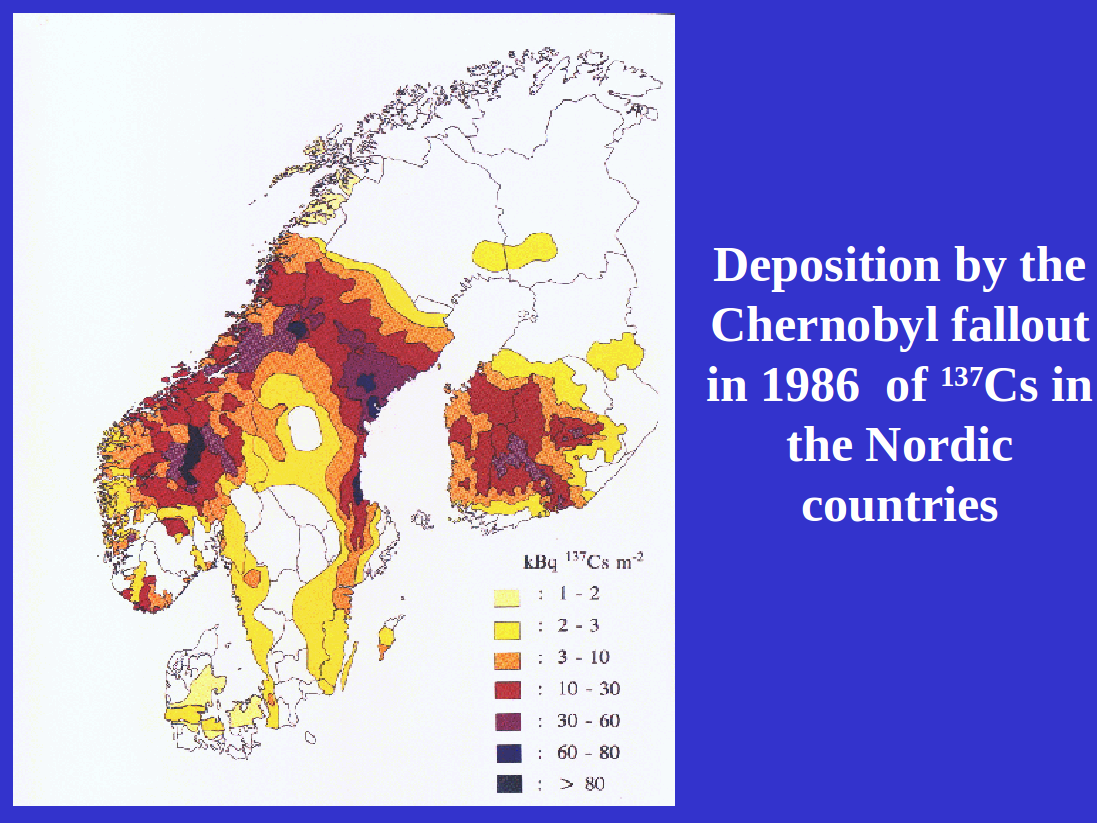
\includegraphics[scale=0.25]{figures/fallout.png}

\end{frame}

\begin{frame}{Examples of doses due to artificial radionuclides}

\centering
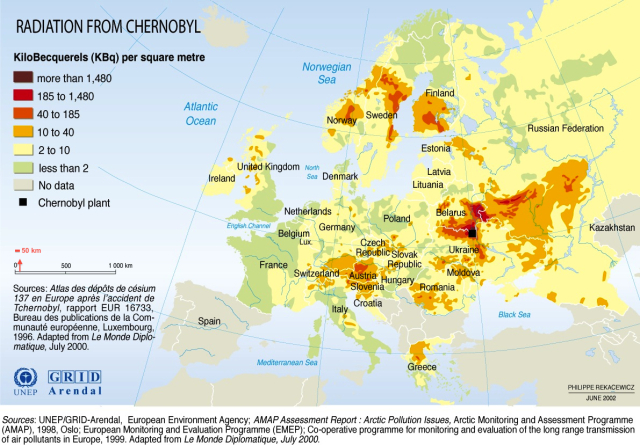
\includegraphics[scale=0.5]{figures/fallouteurope}

\end{frame}

\begin{frame}{Examples of doses due to natural radionuclides}

\centering
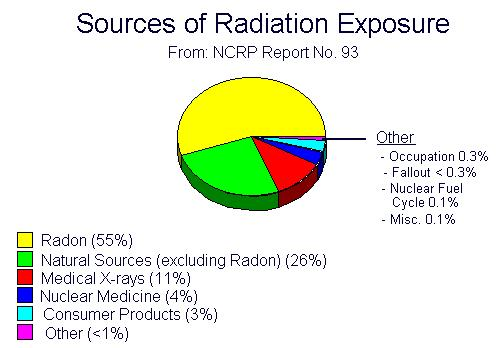
\includegraphics[scale=0.5]{figures/dosespopulation}

\end{frame}

\begin{frame}{Learnings so far}

\begin{alertblock}{Let's remember}

\begin{itemize}

\pause \item Magnitudes use on radioactivity: Exposure (X), Absorbed dose (D), Equivalent dose (H), Effective dose (E)

\pause \item New units: Exposure (R), Absorbed dose (D), Equivalent and effective dose (Sv)

\pause \item Relations between magnitudes: exposure and activity ( exposure rate constant $\Gamma$); activity and equivalent dose (K)

\pause \item Examples of doses due to natural radiation and artificial radiation (radioactive fallout)

\end{itemize}

\end{alertblock}

\end{frame}